\chapter{Supplementary Material for Zero-Field Edge Plasmons in a Magnetic Topological Insulator}
\section{Fabrication Details}
The film used to make the circulator and corresponding Hall bar is seven quintuple layers of \ce{(Cr_{0.12}Bi_{0.26}Sb_{0.62})_2Te3}. We use photolithography to pattern a circular mesa with a diameter of \SI{330}{\micron}. We bake the Megaposit SPR 3612 photoresist at \SI{80}{\celsius} (to avoid possible damage to the film from overheating), and develop with MF CD-30 after exposure. To define the mesa, we etch the surrounding film via Ar ion milling. After patterning the contacts and ground plane with the same photolithographic procedure, we deposit a \SI{5}{\nano\meter} Ti sticking layer followed by \SI{120}{\nano\meter} Au using e-beam evaporation. The capacitive contacts are designed to be \SI{20}{\micron} from the edge of the circular mesa. For the primary device discussed in this work, the relative misalignment of the mesa and contacts is approximately \SI{5}{\micron}.

\clearpage
\section{Supplementary Figures}
\begin{figure}[h]
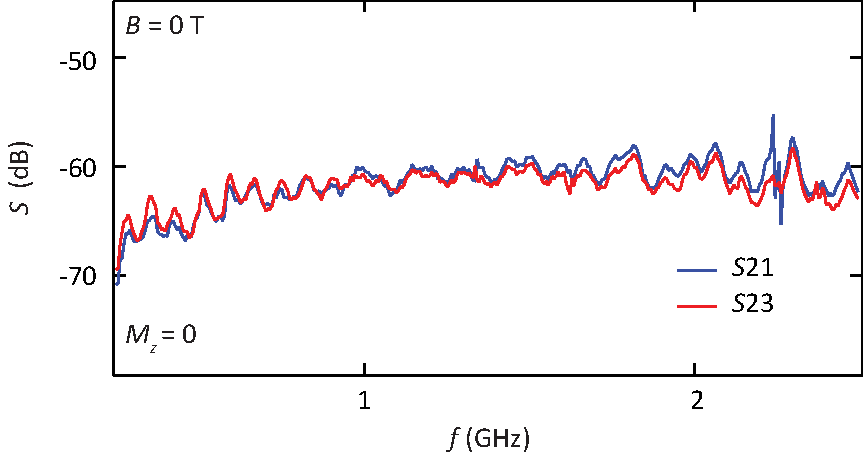
\includegraphics[scale=0.75]{fig_S1QH}
\caption[Microwave transmission prior to sample magnetisation]{Microwave transmission prior to sample magnetisation. $S$-parameter transmission measurements taken prior to device magnetisation at cryostat base temperature of $\sim \SI{20}{\mk}$, and applied port power of \SI{-72}{\dBm}. Traces have been corrected for amplification and attenuation added to the setup in order to provide a measure of insertion loss. Subtracting the bare $S$-parameter responses $S_{23}$ from $S_{21}$ (as shown in Fig.~\ref{fig:fig2_ti} (d)) yields a small residual response at $B=\SI{0}{\tesla}$ about \SI{0}{\decibel}, attributed to slight differences in the line impedances of the two rf setups.}
\label{fig:qah_s1}
\end{figure}

\begin{figure}[h]
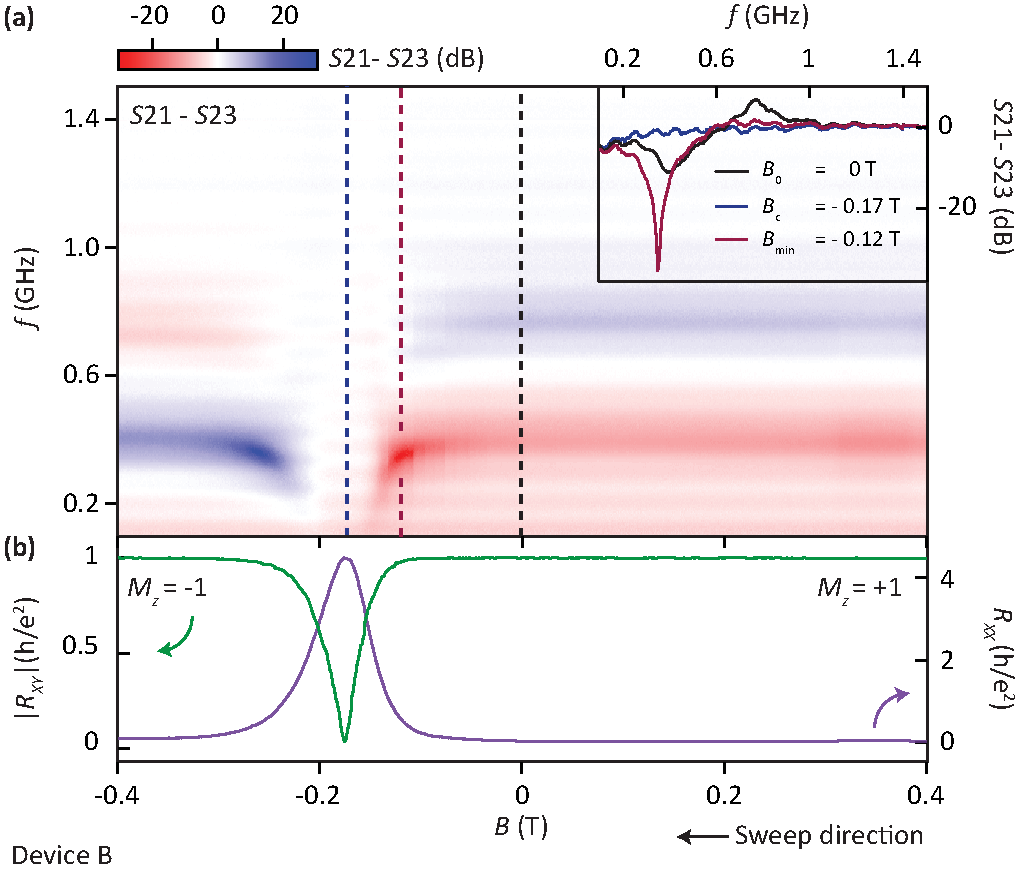
\includegraphics[scale=0.7]{fig_S2QH}
\caption[Power and temperature dependence of TI absorption]{Power and temperature dependence at $M_z = +1$ (a) - (d) Show the effect of temperature and applied microwave port power on $S_{21}$ and $S_{23}$ at $B=\SI{0}{\tesla}$ once the sample has been magnetised in the positive direction, $M_z=+1$. The direction of magnetisation has been reversed with respect to the data in Fig.~\ref{fig:fig4_ti}. In accordance with a reversal of chirality, hot-spots are observed in the normalised $\Delta S_{21}$ plots with both power and cryostat base temperature, corresponding to the $2l$ path in this configuration. Colour bar represents $\Delta S$ (\si{\decibel}).}
\label{fig:qah_s2}
\end{figure}

\begin{figure}[h]
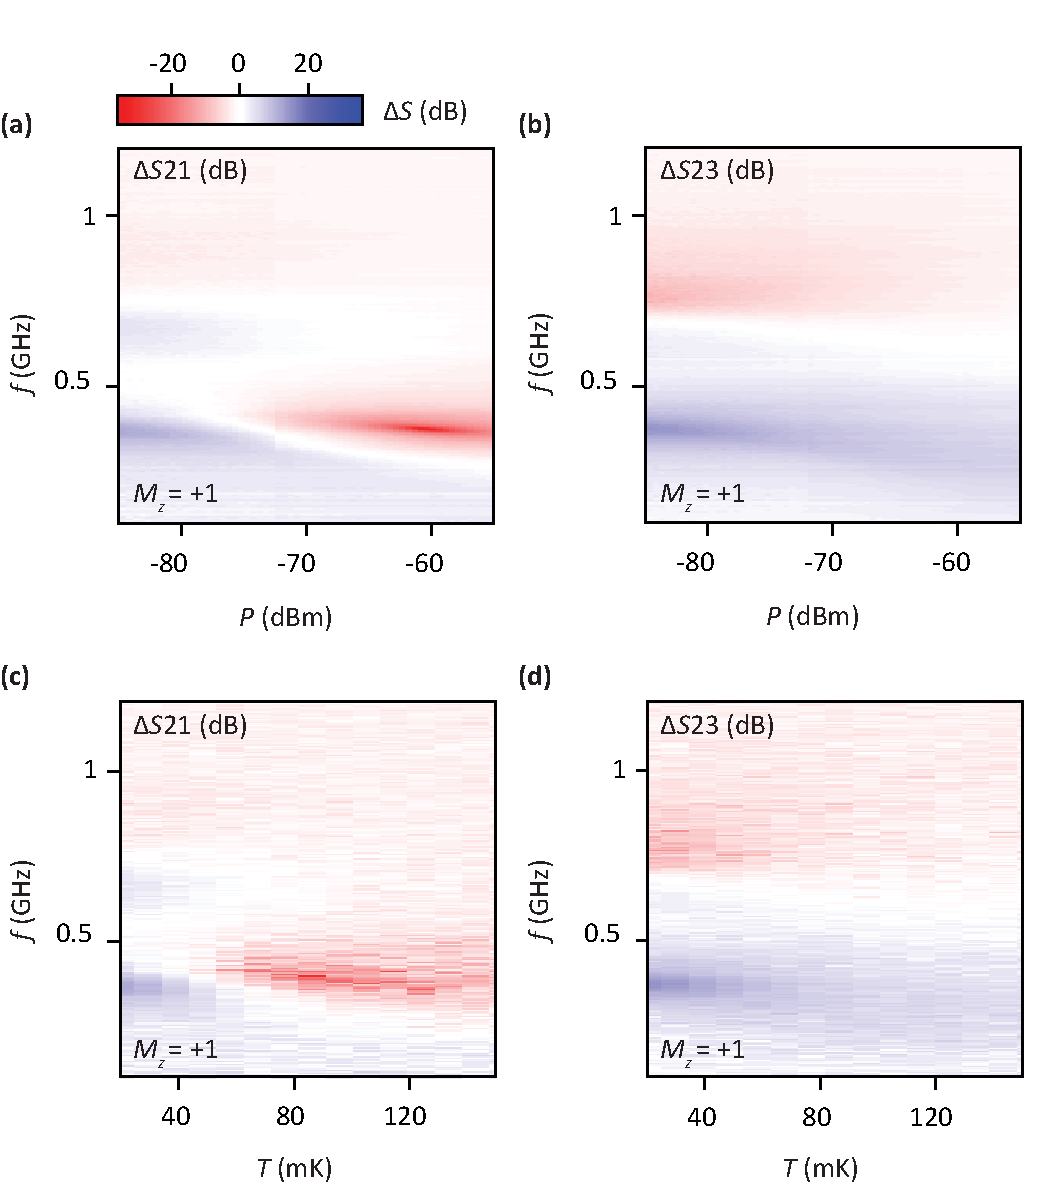
\includegraphics[scale=0.7]{fig_S3QH}
\caption[Secondary TI device]{Secondary device. $S_{21}$-$S_{23}$ microwave spectrum is shown in (a), while Hall bar transport measurements are presented in (b) for a secondary device on a separate growth.  Colour bar shows $S_{21}$-$S_{23}$ in \si{\decibel}. The material comprises 8 quintuple layers of \ce{(Cr_{0.12}Bi_{0.26}Sb_{0.62})_2Te3}, with fabrication methods and circulator geometry nominally identical to the device outlined in Sec.\ref{sec:spinhallcirc}. Inset shows cuts taken at constant magnetic field values corresponding to dashed lines in (a).}
\label{fig:qah_s3}
\end{figure}
